% Standalone pgfplots: the H_1211 dual-substrate scale-recheck ladder.
% All numbers verbatim from .verdicts/1211_dual_substrate_scaleup/H_1211.txt
% (3-seed means). LEFT = AXIS-T (stream length 1x/10x/100x): the density
% NOVEL/REPEAT separation STRENGTHENS while the trajectory WALK/WALK_SHUF
% separation COLLAPSES through the frozen 1.5 bar; density blind stays ~1.0.
% RIGHT = AXIS-P (alphabet N_PROTO 24/64/128 at fixed toy T): the trajectory
% separation is RESTORED + sharpened, confirming small-alphabet saturation.
\documentclass[border=4pt]{standalone}
\usepackage{pgfplots}
\pgfplotsset{compat=1.18}
\begin{document}
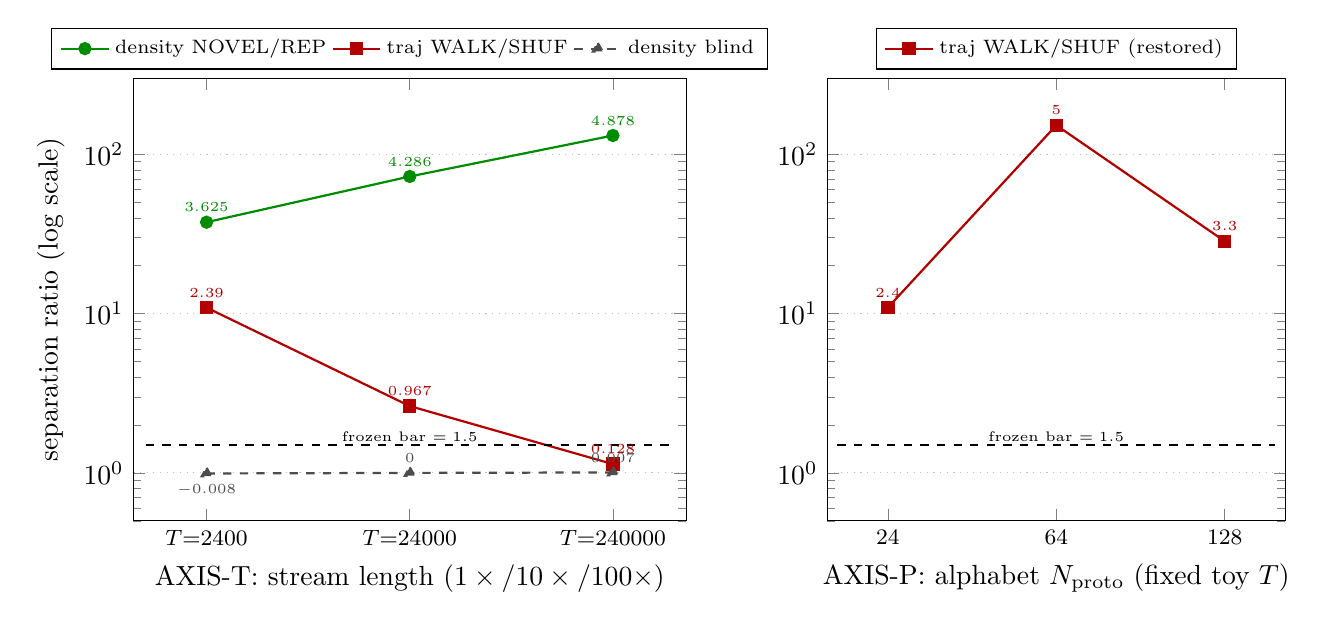
\begin{tikzpicture}

% ---------- LEFT: AXIS-T (stream length) ----------
\begin{axis}[
    name=axisT,
    width=8.6cm, height=7.2cm,
    ymode=log,
    ymin=0.5, ymax=300,
    xtick={1,2,3},
    xticklabels={$T{=}2400$, $T{=}24000$, $T{=}240000$},
    x tick label style={font=\footnotesize},
    xlabel={AXIS-T: stream length ($1\times/10\times/100\times$)},
    ylabel={separation ratio (log scale)},
    ymajorgrids, grid style={dotted},
    legend style={font=\scriptsize, at={(0.5,1.02)}, anchor=south, legend columns=3},
    enlarge x limits=0.18,
    nodes near coords, nodes near coords style={font=\tiny, /pgf/number format/fixed, /pgf/number format/precision=3},
]
\addplot[green!55!black, mark=*, thick] coordinates {(1,37.538) (2,72.714) (3,131.429)};
\addplot[red!70!black, mark=square*, thick] coordinates {(1,10.916) (2,2.629) (3,1.136)};
\addplot[gray!60!black, mark=triangle*, thick, dashed] coordinates {(1,0.992) (2,1.000) (3,1.007)};
\draw[dashed, thick, black] (axis cs:0.7,1.5) -- (axis cs:3.3,1.5)
  node[pos=0.5, above, font=\tiny, fill=white, inner sep=1pt] {frozen bar $=1.5$};
\legend{density NOVEL/REP, traj WALK/SHUF, density blind}
\end{axis}

% ---------- RIGHT: AXIS-P (alphabet N_PROTO) ----------
\begin{axis}[
    name=axisP,
    at={(axisT.right of east)}, anchor=left of west,
    width=7.4cm, height=7.2cm,
    ymode=log,
    ymin=0.5, ymax=300,
    xtick={1,2,3},
    xticklabels={$24$, $64$, $128$},
    x tick label style={font=\footnotesize},
    xlabel={AXIS-P: alphabet $N_{\mathrm{proto}}$ (fixed toy $T$)},
    ymajorgrids, grid style={dotted},
    legend style={font=\scriptsize, at={(0.5,1.02)}, anchor=south, legend columns=1},
    enlarge x limits=0.18,
    nodes near coords, nodes near coords style={font=\tiny, /pgf/number format/fixed, /pgf/number format/precision=1},
]
\addplot[red!70!black, mark=square*, thick] coordinates {(1,10.916) (2,152.500) (3,28.500)};
\draw[dashed, thick, black] (axis cs:0.7,1.5) -- (axis cs:3.3,1.5)
  node[pos=0.5, above, font=\tiny, fill=white, inner sep=1pt] {frozen bar $=1.5$};
\legend{traj WALK/SHUF (restored)}
\end{axis}

\end{tikzpicture}
\end{document}
